%; whizzy document
% latex beamer presentation.
% platex, latex-beamer $B$G%3%s%Q%$%k$9$k$3$H$rA[Dj!%(B 

\documentclass[cjk,dvipdfm]{beamer}
\usetheme{Warsaw}
%  preview (shell-command (concat "xpdf " (replace-regexp-in-string "tex$" "pdf"(buffer-file-name)) "&"))
%  presentation (shell-command (concat "xpdf -fullscreen " (replace-regexp-in-string "tex$" "pdf"(buffer-file-name)) "&"))

\title{Mactel Debian $B$N?<1s$J$k@$3&(B}
%\title[Debian $BJY6/2q%/%$%:LdBj(B]{Debian$BJY6/2q%/%$%:(B}
\subtitle{2006$BG/(B7$B7n(B15$BF|HG(B}
\author{$B>e@n(B}
\date{2006$BG/(B7$B7n(B15$BF|(B}

% $B;0BrLdBjMQ(B
\newcounter{santakucounter}
\newcommand{\santaku}[5]{%
\addtocounter{santakucounter}{1}
\frame{\frametitle{$BLdBj(B\arabic{santakucounter}. #1}
%$BLdBj(B\arabic{santakucounter}. #1
\begin{minipage}[t]{0.7\hsize}
 \begin{itemize}
 \item $B""(B A #2\\
 \item $B""(B B #3\\
 \item $B""(B C #4\\
 \end{itemize}
\end{minipage}
}
\frame{\frametitle{$BLdBj(B\arabic{santakucounter}. #1}
%$BLdBj(B\arabic{santakucounter}. #1
\begin{minipage}[t]{0.7\hsize}
\begin{itemize}
\item $B""(B A #2\\
\item $B""(B B #3\\
\item $B""(B C #4\\
\end{itemize}
\end{minipage}
\begin{minipage}[t]{0.2\hsize}
$BEz$($O(B:


\vspace{1cm}

{\huge \hspace{1cm}#5}
\end{minipage}}
}


\begin{document}
\frame{\titlepage{}}

\section{DWNQuiz}
%% debianmeetingresume200607.tex$B$+$i0J2<%3%T!<(B

\section{MactelLinux}
\begin{frame}
\frametitle{MactelLinux $B8=>u$N35MW(B}
\begin{center}
\begin{minipage}{0.5\hsize}
  \begin{itemize}
 \item$B!!?7%"!<%-%F%/%A%c(B\\
       $B5/F0ItJ,$O(BEFI
 \end{itemize}
\end{minipage}
\end{center}
\end{frame}
\begin{frame}
\frametitle{EFI$B$H$$$&J!2;(B}

\begin{tabular}[t]{|p{8em}|p{8em}|p{8em}|}
\hline
 & BIOS & EFI \\
\hline
$B%Q!<%F%#%7%g%s(B & MBR:4$B8D!!(B($B!V3HD%!W2DG=(B) & GPT: 128 \\
\hline
$B%U%!%$%k%7%9%F%`(B &$B!!Kb7"(B & FAT $B$rFI$a$k(B \\
\hline
$B<B9T%U%)!<%^%C%H(B & $B$J$K$=$l(B? & PE32+$B7A<0$N<B9T%U%!%$%k(B\\
\hline
\end{tabular}
\end{frame}

\begin{frame}
\frametitle{$B5/F0%7!<%1%s%9(B}
\begin{minipage}[t]{0.4\hsize}
% dotty -Tps -o bootchain.ps bootchain.dot
\includegraphics[height=1\hsize]{image200607/bootchain.ps}
\end{minipage}
\begin{minipage}[t]{0.58\hsize}
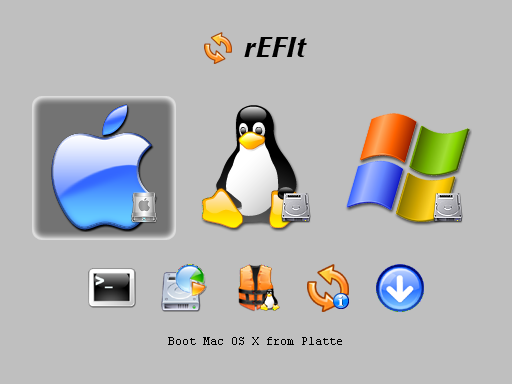
\includegraphics[width=1\hsize]{image200607/screen1.png}
\end{minipage}
\end{frame}

\begin{frame}
\frametitle{EFI$B%3%^%s%I%i%$%s(B}

MS DOS $BIwL#$N%3%^%s%I%i%$%s$,MxMQ$G$-$k$h$&$K$J$k!#(B\\
$B%V!<%H%m!<%@0JA0$NCJ3,$G%3%^%s%I%i%$%s$,MxMQ$G$-$k$h$&$K(B!

EFI$>$ fs0:\\
EFI fs0:$>$ cd EFI\\
EFI fs0:$\backslash{}$EFI$>$ cd dancer\\
EFI fs0:$\backslash{}$EFI$\backslash{}$dancer$>$ cd refit\\
EFI fs0:$\backslash{}$EFI$\backslash{}$dancer$\backslash{}$refit$>$ dir\\
refit.efi\\
 EFI fs0:$\backslash{}$EFI$\backslash{}$debian$\backslash{}$refit$>$ refit

\end{frame}

\begin{frame}
\frametitle{$B$G$-$?$3$H(B}
\begin{itemize}
 \item rEFIt$B$r(BDebian$B>e$G%3%s%Q%$%k$G$-$k$h$&$K(B
 \item refit Debian$B%Q%C%1!<%8$N:n@.!"%"%C%W%m!<%I(B (375999)
 \item $B$=$l$C$]$/F0:n;n83(B
 \item gptsync$B%3%^%s%I$NDs6!(B
\end{itemize}
\end{frame}

\begin{frame}
\frametitle{$B$G$-$F$J$$$3$H(B}
\begin{itemize}
 \item $B%$%s%9%H!<%k<jK!$N3NN)(B\\
       MacOSX$B$N(Bbless $B%3%^%s%I$K0MB8$7$J$$J}K!$,$J$$(B
 \item debian-installer$B$X$NE}9g(B
 \item rEFIt$B$G%3%s%Q%$%k$G$-$J$$%D!<%kB??t(B\\
       gptsync.efi$B$,F0:n$7$F$$$J$$(B\\
       gnu-efi$B$N(Befilib$B$,$I$&$b8E$$$h$&$@(B(376000)
 \item $B%P%$%J%jG[I[$5$l$F$$$k%D!<%k$NH/8+(B($B%=!<%9$O$I$3(B?)
 \item elilo $B$,$&$^$/$&$4$+$J$$(B (376002)
 \item Debian$B$N(B2.6.16/2.6.17$B%+!<%M%k$O(B
       $B$h$/%+!<%M%k%Q%K%C%/$r$*$3$9(B\\
       (Linus$B$N(B7$B7n(B2$BF|$N(Bgit$B%D%j!<$O0BDjF0:n!"(BMactel$BMQ$N%Q%C%A$,B??t%^!<%8(B
       $B$5$l$F$$$k$h$&$J$N$G$*A&$a(B)
\end{itemize}
\end{frame}
\begin{frame}
\frametitle{MBR vs GPT}
\begin{minipage}[t]{0.65\hsize} 
{\scriptsize
 Disk /dev/sda: 80.0 GB, 80026361856 bytes\\
255 heads, 63 sectors/track, 9729 cylinders\\
Units = cylinders of 16065 * 512 = 8225280 bytes\\

   Device Boot      Start         End      Blocks   Id  System\\
/dev/sda1               1          26      204819+  ee  EFI GPT\\
/dev/sda2              26        2637    20971520   af  Unknown\\
/dev/sda3   *        2637        2758      976563   ef  EFI (FAT-12/16/32)\\
/dev/sda4            2758        5190    19531250+  ef  EFI (FAT-12/16/32)\\
}
\end{minipage}
\begin{minipage}[t]{0.30\hsize}
{\small
 major minor  $\sharp{}$blocks  name\\

   8     0   78150744 sda\\
   8     1     204800 sda1\\
   8     2   20971520 sda2\\
   8     3     976563 sda3\\
   8     4   19531250 sda4\\
   8     5    2929688 sda5\\
}
\end{minipage}
\end{frame}

\begin{frame}
 \frametitle{}
\begin{itemize}
 \item hfsplus -- HFS plus $B%U%!%$%k%7%9%F%`(B
 \item hfsplus $B%+!<%M%k%b%8%e!<%k(B -- HFS plus $B%U%!%$%k%7%9%F%`(B
 \item hfsutils -- HFS 
 \item \url{http://ipodlinux.org/Installation_from_Linux_Hfsplus}
 \item \url{http://darwinsource.opendarwin.org/tarballs/apsl/bless-37.tar.gz}
\end{itemize}
\end{frame}


\end{document}